% \section{Appendix}

% \eb{We present model details below to fully illustrate of the proposed semantics, and show that interpreted strength is a linear function of utterance cost (Fig \ref{model-heights}).
% While it should be possible to predict participants' responses in these studies directly from the semantics, it is sufficient to use more standard regression models to measure the linear relationship between communicative cost and interpretation strength.
% We therefore modeled the human data using regression models.
% The corresponding coefficients for these regression models are shown in Tables \ref{regressions1a}, \ref{regressions1b}, \ref{regressions2}, \ref{regressions3}, and \ref{regressions4}.}

\begin{appendices}

\counterwithin{figure}{section}
\counterwithin{table}{section}


\section{Pragmatic Model \label{app:model}}

\citeA{lassiter_context_2013}'s model of scalar adjectives belongs to the family of Rational Speech Act (RSA) models in which speaker and listener communicate by  reasoning about each other's goals and inferences (\citeNP{frank_predicting_2012, goodman_knowledge_2013}; for related models, see also \citeNP{franke_quantity_2011, russell_probabilistic_2012}). 
These models have been shown to account for a number of key phenomena in pragmatics. The adjective model accounts for uncertainty about the adjectival threshold by including a semantic variable, which the pragmatic listener infers at the same time that she infers the speaker's intended meaning. 

RSA models begin with a literal listener, which captures the semantic denotation of sentences. 
We assume adjective phrases with the same scale and polarity have the same denotation. For example, \w{expensive}, \w{very expensive} and \w{phenomenally expensive} all denote: $\lambda x . \text{price}(x) > \theta_i$. %unpack?
However, every adjective phrase has its own threshold variable $\theta_i$,\footnote{%
%
Other versions of this model could easily be imagined in which the threshold for an adjective phrase is determined by the basic threshold for the adjective and \eb{some transformation on that threshold caused by the intensifier. 
For example, \cite{cliff1959adverbs} argue that intensifying adverbs operate on adjectives meanings through scalar multiplication.
% (e.g. multiplication, addition, etc.)
If, as in multiplication, the transformation is regular, with a single parameter needing to be inferred for each intensifier, and if the values of these parameters are inferred for each adjective phrase, then such a model would be functionally equivalent to the one we describe here.%
}
%
} together notated $\vec{\theta}$, allowing their meanings to differ.
Given an utterance $u_i$ (e.g. an \w{expensive laptop} or a \w{very expensive laptop}) and a set of thresholds, a literal listener $L_0$ will use Bayesian inference to update his prior beliefs $P(d)$ about the degree $d$ (e.g. the laptop's price) given that the degree is greater than the threshold for that utterance.

$$P_{L_0}(d|u_i, \theta_i) \propto P(d) \cdot \delta_{d > \theta_i}$$

A speaker with the goal of communicating some actual degree $d$ assigns a utility $\mathbb{U}(u_i|d)$ to each utterance such that he prefers utterances which will inform the literal listener, but avoids utterance cost, $C(u_i)$:

$$\mathbb{U}(u_i | d, \vec{\theta}) =  \ln\left(P_{L_0}(d | u_i, \theta_i) \right) - C(u_i) $$

Given a set of alternative utterances (e.g. the speaker might be choosing between saying \w{very expensive} as opposed to \w{expensive} or \w{extremely expensive}, or saying nothing at all), the speaker $S_1$ will choose utterances according to a softmax decision rule \cite{sutton_reinforcement_2011} with optimality parameter $\lambda$, so that:

$$ P_{S_1}(u_i | d, \vec{\theta}) \propto e^{\lambda \mathbb{U}(u_i | d, \vec{\theta})} $$

A pragmatic listener $L_1$ uses the prior probability, $P(d)$, of different degrees, along with knowledge of the cost of each utterance, in order to guess both the thresholds for each utterance and which degree the speaker intended to communicate\footnote{We assume a uniform prior on thresholds $\theta_i$.}:

$$ P_{L_1}(d, \vec{\theta} | u_i) \propto P(d) \cdot P_{S_1}(u_i | d, \vec{\theta}) $$

We simulated such a model with three alternative adjective phrases (i.e.~three intensifiers) with costs of $1$, $5$, and $10$. We also included a null utterance, with trivial meaning (always true) and cost of $0$. The prior distribution of degrees along this adjective's scale (which we will discuss as ``prices'' for concreteness and consistency with our Experiment 1) was a gaussian peaked at $0$.
We used an optimality parameter of $\lambda=5$ in our simulation. 

Though the literal semantics are identical (but permitting different threshold parameters), the different phrases received different interpretations: the more costly intensifiers corresponded to less probable, more extreme prices (Figure ~\ref{model}).
This can be seen as an M-implicature: more costly intensifiers are assigned stronger, less probable, meanings. 
The model therefore predicts an association between intensifier meaning and utterance cost (see \citeA{bergen_pragmatic_2014} for other M-implicature models within the RSA framework).


\begin{figure}[htb]
\begin{center}
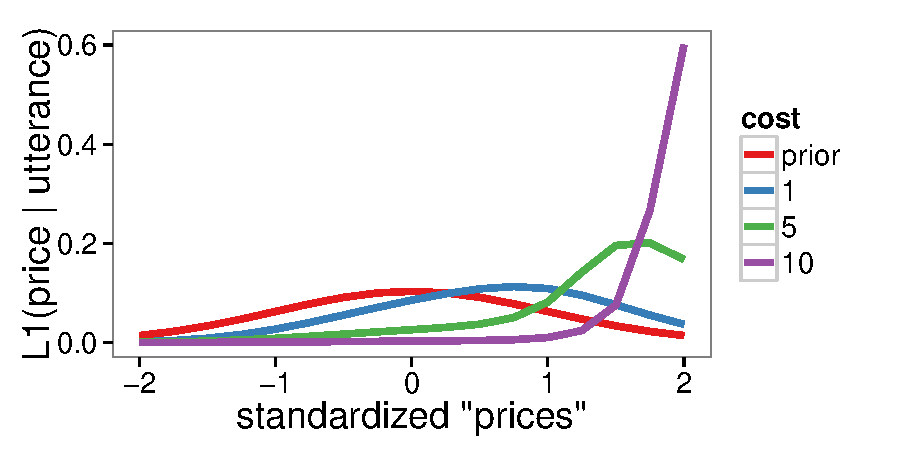
\includegraphics[width=0.4\textwidth]{model_results.pdf}
\end{center}
\caption{Modeling intensifiers as M-implicature: more costly intensifiers correspond to more extreme meanings.} 
\label{model}
\end{figure}

To assess the quantitative relationship between cost and meaning, we ran a second simulation, identical as the first except using 6 different utterance costs (or ``intensifiers'').
The quantitative form predicted by the model is a approximately linear (Figure \ref{model-heights}).
It is this simple prediction that we explore in the main text.


\begin{figure}[htb]
\begin{center}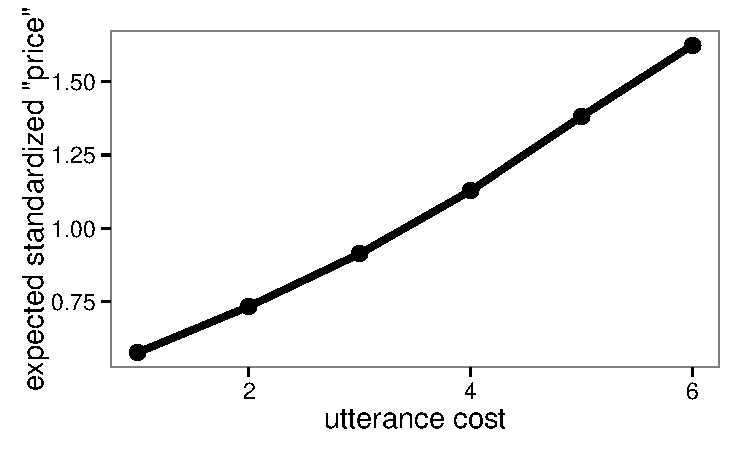
\includegraphics[width=0.35\textwidth]{height-by-cost.pdf}
\end{center}
\caption{Model prediction of expected price as cost of intensifier increases, based on intensifiers evenly spaced in cost. The relationship is approximately linear.} 
\label{model-heights}
\end{figure}


\section{Study 1a Regressions}

Below, we present results of linear mixed-effects models of scaled responses in Study 1a as a function of length in syllables and surprisal.
Model 1 includes raw predictors.
In Model 2, we replace the length predictor by the residuals when length is modeled as a linear function of surprisal.
In Model 3, we replace the surprisal predictor by the residuals when surprisal is modeled as a linear function of length.
Finally, we present results of likelihood ratio tests when each of the predictors is removed from the full model.

\vspace{4mm}

\noindent
\footnotesize{
\begin{tabular}{r|cccc}
\hline
\hline
\multicolumn{5}{c}{\textbf{Study 1a Regression Results}} \\
\hline
\hline
\multicolumn{5}{c}{Model 1: Colinear Predictors} \\
& Estimate & se & $t$ & $p$ \\
\hline
Length & 0.133 & 0.077 & 1.72 & 0.094 \\
Surprisal & 0.106 & 0.031 & 3.41 & 0.002 \\
\hline
\hline
\multicolumn{5}{c}{Model 2: Length, residualized by Surprisal} \\
& Estimate & se & $t$ & $p$ \\
\hline
Length\textsubscript{resid} & 0.133 & 0.077 & 1.72 & 0.094 \\
Surprisal & 0.120 & 0.030 & 3.98 & $<0.001$ \\
\hline
\hline
\multicolumn{5}{c}{Model 3: Surprisal, residualized by Length} \\
& Estimate & se & $t$ & $p$ \\
\hline
Length & 0.202 & 0.075 & 2.69 & 0.010 \\
Surprisal\textsubscript{resid} & 0.106 & 0.031 & 3.41 & 0.002 \\
\hline
\hline
\multicolumn{5}{c}{Model Comparison:} \\
\multicolumn{5}{c}{Predictors removed from Model 1} \\
& $\chi^2$ & $p$ \\
\hline
Length & 13.70 & 0.003 \\
Surprisal & 17.05 & 0.001 \\
\hline
\hline
\end{tabular}
}



\section{Study 1b Regressions}

Below, we present results of linear mixed-effects models of scaled responses in Study 1b as a function of length in syllables and surprisal.
Model 1 includes raw predictors.
In Model 2, we replace the length predictor by the residuals when length is modeled as a linear function of surprisal.
In Model 3, we replace the surprisal predictor by the residuals when surprisal is modeled as a linear function of length.
Finally, we present results of likelihood ratio tests when each of the predictors is removed from the full model.

\vspace{4mm}

\noindent
\footnotesize{
\begin{tabular}{r|cccc}
\hline
\hline
\multicolumn{5}{c}{\textbf{Study 1b Regression Results}} \\
\hline
\hline
\multicolumn{5}{c}{Model 1: Colinear Predictors} \\
& Estimate & se & $t$ & $p$ \\
\hline
Length & 0.055 & 0.054 & 1.02 & 0.311 \\
Surprisal & 0.107 & 0.033 & 3.26 & 0.002 \\
\hline
\hline
\multicolumn{5}{c}{Model 2: Length, residualized by Surprisal} \\
& Estimate & se & $t$ & $p$ \\
\hline
Length\textsubscript{resid} & 0.055 & 0.054 & 1.02 & 0.311 \\
Surprisal & 0.128 & 0.026 & 4.96 & $<0.001$ \\
\hline
\hline
\multicolumn{5}{c}{Model 3: Surprisal, residualized by Length} \\
& Estimate & se & $t$ & $p$ \\
\hline
Length & 0.166 & 0.042 & 3.93 & $<0.001$ \\
Surprisal\textsubscript{resid} & 0.107 & 0.033 & 3.26 & 0.002 \\
\hline
\hline
\multicolumn{5}{c}{Model Comparison:} \\
\multicolumn{5}{c}{Predictors removed from Model 1} \\
& $\chi^2$ & $p$ \\
\hline
Length & 11.57 & 0.009 \\
Surprisal & 30.32 & $<0.001$ \\
\hline
\hline
\end{tabular}
}



\section{Study 2 Regressions}

Below, we present results of linear mixed-effects models of rankings in Study 2 as a function of length in syllables and surprisal.
Model 1 includes raw predictors.
In Model 2, we replace the length predictor by the residuals when length is modeled as a linear function of surprisal.
In Model 3, we replace the surprisal predictor by the residuals when surprisal is modeled as a linear function of length.
In Model 4, we add interactions for adjectives.
Finally, we present results of likelihood ratio tests when each of the length and surprisal predictors are removed from Model 1.

\vspace{4mm}

\noindent
\footnotesize{
\begin{tabular}{r|cccc}
\hline
\hline
\multicolumn{5}{c}{\textbf{Study 2 Regression Results}} \\
\hline
\hline
\multicolumn{5}{c}{Model 1: Colinear Predictors} \\
& Estimate & se & $t$ & $p$ \\
\hline
Surprisal & 0.164 & 0.016 & 10.13 & $<0.001$ \\
Length & 0.243 & 0.041 & 5.89 & $<0.001$ \\
\hline
\hline
\multicolumn{5}{c}{Model 2: Length, residualized by Surprisal} \\
& Estimate & se & $t$ & $p$ \\
\hline
Surprisal & 0.190 & 0.016 & 11.66 & $<0.001$ \\
Length\textsubscript{resid} & 0.243 & 0.041 & 5.89 & $<0.001$ \\
\hline
\hline
\multicolumn{5}{c}{Model 3: Surprisal, residualized by Length} \\
& Estimate & se & $t$ & $p$ \\
\hline
Length & 0.350 & 0.041 & 8.46 & $<0.001$ \\
Surprisal\textsubscript{resid} & 0.164 & 0.016 & 10.13 & $<0.001$ \\
\hline
\hline
\multicolumn{5}{c}{Model 4: With Adjective Interaction} \\
& Estimate & se & $t$ & $p$ \\
\hline
Surprisal & 0.074 & 0.030 & 2.48 & 0.013 \\
Length & 0.318 & 0.087 & 3.66 & $<0.001$ \\
\multicolumn{1}{l|}{Surprisal:Adj} & & & & \\
\multicolumn{1}{l|}{\ \ Adj=Tall} & 0.188 & 0.045 & 4.14 & $<0.001$ \\
\multicolumn{1}{l|}{\ \ Adj=Expensive} & 0.170 & 0.047 & 3.66 & $<0.001$ \\
\multicolumn{1}{l|}{\ \ Adj=Old} & 0.037 & 0.043 & 0.85 & 0.393 \\
\multicolumn{1}{l|}{Length:Adj} & & & & \\
\multicolumn{1}{l|}{\ \ Adj=Tall} & -0.103 & 0.121 & -0.86 & 0.393 \\
\multicolumn{1}{l|}{\ \ Adj=Expensive} & -0.100 & 0.119 & -0.84 & 0.400 \\
\multicolumn{1}{l|}{\ \ Adj=Old} & -0.092 & 0.119 & -0.78 & 0.438 \\
\hline
\hline
\multicolumn{5}{c}{Model Comparison:} \\
\multicolumn{5}{c}{Predictors removed from Model 1} \\
& $\chi^2$ & $p$ \\
\hline
Length & 34.69 & $<0.001$ \\
Surprisal & 108.08 & $<0.001$ \\
\hline
\hline
\end{tabular}
}



\section{Study 3 Regressions}


Below, we present results of linear mixed-effects models of scaled responses in Study 3's replication portion as a function of length in syllables and surprisal.
Model 1 includes raw predictors.
In Model 2, we replace the length predictor by the residuals when length is modeled as a linear function of surprisal.
In Model 3, we replace the surprisal predictor by the residuals when surprisal is modeled as a linear function of length.
Finally, we present results of likelihood ratio tests when each of the predictors is removed from the full model.

\vspace{4mm}

\noindent
\footnotesize{
\begin{tabular}{r|cccc}
\hline
\hline
\multicolumn{5}{c}{\textbf{Study 3 (replication portion) Regression Results}} \\
\hline
\hline
\multicolumn{5}{c}{Model 1: Colinear Predictors} \\
& Estimate & se & $t$ & $p$ \\
\hline
Length & 0.194 & 0.095 & 2.05 & 0.085 \\
Surprisal & 0.140 & 0.056 & 2.49 & 0.041 \\
\hline
\hline
\multicolumn{5}{c}{Model 2: Length, residualized by Surprisal} \\
& Estimate & se & $t$ & $p$ \\
\hline
Length\textsubscript{resid} & 0.194 & 0.095 & 2.05 & 0.085 \\
Surprisal & 0.182 & 0.052 & 3.47 & 0.010 \\
\hline
\hline
\multicolumn{5}{c}{Model 3: Surprisal, residualized by Length} \\
& Estimate & se & $t$ & $p$ \\
\hline
Length & 0.286 & 0.088 & 3.24 & 0.016 \\
Surprisal\textsubscript{resid} & 0.140 & 0.056 & 2.49 & 0.041 \\
\hline
\hline
\multicolumn{5}{c}{Model Comparison:} \\
\multicolumn{5}{c}{Predictors removed from Model 1} \\
& $\chi^2$ & $p$ \\
\hline
Length & 8.30 & 0.040 \\
Surprisal & 39.19 & $<0.001$ \\
\hline
\hline
\end{tabular}
}

\vspace{4mm}

Below, we present results of regressions predicting scaled responses for novel intensifiers in Study 3.

\vspace{4mm}

\noindent
\footnotesize{
\begin{tabular}{r|cccc}
\hline
\hline
\multicolumn{5}{c}{\textbf{Study 3 (novel intensifiers) Regression Results}} \\
\hline
\hline
\multicolumn{5}{c}{Model 1: Short/Long Novel Adverbs} \\
& Estimate & se & $t$ & $p$ \\
\hline
(Intercept) &  0.110 & 0.366 & 0.299 & 0.768 \\
Length &  0.538 & 0.195 & 2.757 & 0.011 \\
 % 0.76780306  0.01090199
\hline
\hline
\multicolumn{5}{c}{Model 2: Length and Root Type} \\
& Estimate & se & $t$ & $p$ \\
\hline
(Intercept) & 0.100  & 0.197 & 0.510 & 0.615 \\
Length & 0.540  & 0.195 &   2.772 & 0.011 \\
Ratum/other & -0.371  & 0.143 &  -2.601 & 0.016 \\
Lopus/Bugorn &  0.073  & 0.235 &   0.311 & 0.759 \\
\hline
\hline
\end{tabular}
}

\section{Study 4 Regressions}

Below, we present results of regression predicting rankings for novel intensifiers in Study 4.

\vspace{4mm}

\noindent
\footnotesize{
\begin{tabular}{r|cccc}
\hline
\hline
\multicolumn{5}{c}{\textbf{Study 4 (novel intensifiers) Regression Results}} \\
\hline
\hline
\multicolumn{5}{c}{Model 1: Short/Long Novel Adverbs} \\
& Estimate & se & $z$ & $p$ \\
\hline
Length & 0.70 & 0.253 & 2.79 & 0.005 \\
\hline
\hline
\multicolumn{5}{c}{Model 2: Length and Root Type} \\
& Estimate & se & $z$ & $p$ \\
\hline
Length       &  0.757 & 0.263 &  2.88 & 0.004 \\
Ratum/other  & -0.047 & 0.172 & -0.27 & 0.786 \\ 
Lopus/Bugorn & -0.518 & 0.324 & -1.60 & 0.110 \\
\hline
\hline
\end{tabular}
} 

\vspace{4mm}

Below, we present results of linear mixed-effects models of rankings in Study 4's replication portion as a function of length in syllables and surprisal.
Model 1 includes raw predictors.
In Model 2, we replace the length predictor by the residuals when length is modeled as a linear function of surprisal.
In Model 3, we replace the surprisal predictor by the residuals when surprisal is modeled as a linear function of length.
Finally, we present results of likelihood ratio tests when each of the predictors is removed from the full model.

\vspace{4mm}

\noindent
\footnotesize{
\begin{tabular}{r|cccc}
\hline
\hline
\multicolumn{5}{c}{\textbf{Study 4 (replication portion) Regression Results}} \\
\hline
\hline
\multicolumn{5}{c}{Model 1: Colinear Predictors} \\
& Estimate & se & $t$ & $p$ \\
\hline
Surprisal & 0.447 & 0.032 & 13.88 & $<0.001$ \\
Length & 0.581 & 0.054 & 10.74 & $<0.001$ \\
\hline
\hline
\multicolumn{5}{c}{Model 2: Length, residualized by Surprisal} \\
& Estimate & se & $t$ & $p$ \\
\hline
Surprisal & 0.573 & 0.037 & 15.54 & $<0.001$ \\
Length\textsubscript{resid} & 0.581 & 0.054 & 10.74 & $<0.001$ \\
\hline
\hline
\multicolumn{5}{c}{Model 3: Surprisal, residualized by Length} \\
& Estimate & se & $t$ & $p$ \\
\hline
Length & 0.875 & 0.063 & 13.94 & $<0.001$ \\
Surprisal\textsubscript{resid} & 0.447 & 0.032 & 13.88 & $<0.001$ \\
\hline
\hline
\multicolumn{5}{c}{Model Comparison:} \\
\multicolumn{5}{c}{Predictors removed from Model 1} \\
& $\chi^2$ & $p$ \\
\hline
Length & 130.33 & $<0.001$ \\
Surprisal & 231.57 & $<0.001$ \\
\hline
\hline
\end{tabular}
}



% \begin{table}
% \caption{Study 1b Regression Results}
% \begin{tabular}{ccccc}
% \hline
% \hline
% \hline
% \hline
% \end{tabular}
% \label{regressions}
% \end{table}

\begin{figure}[hbt]
\begin{center}
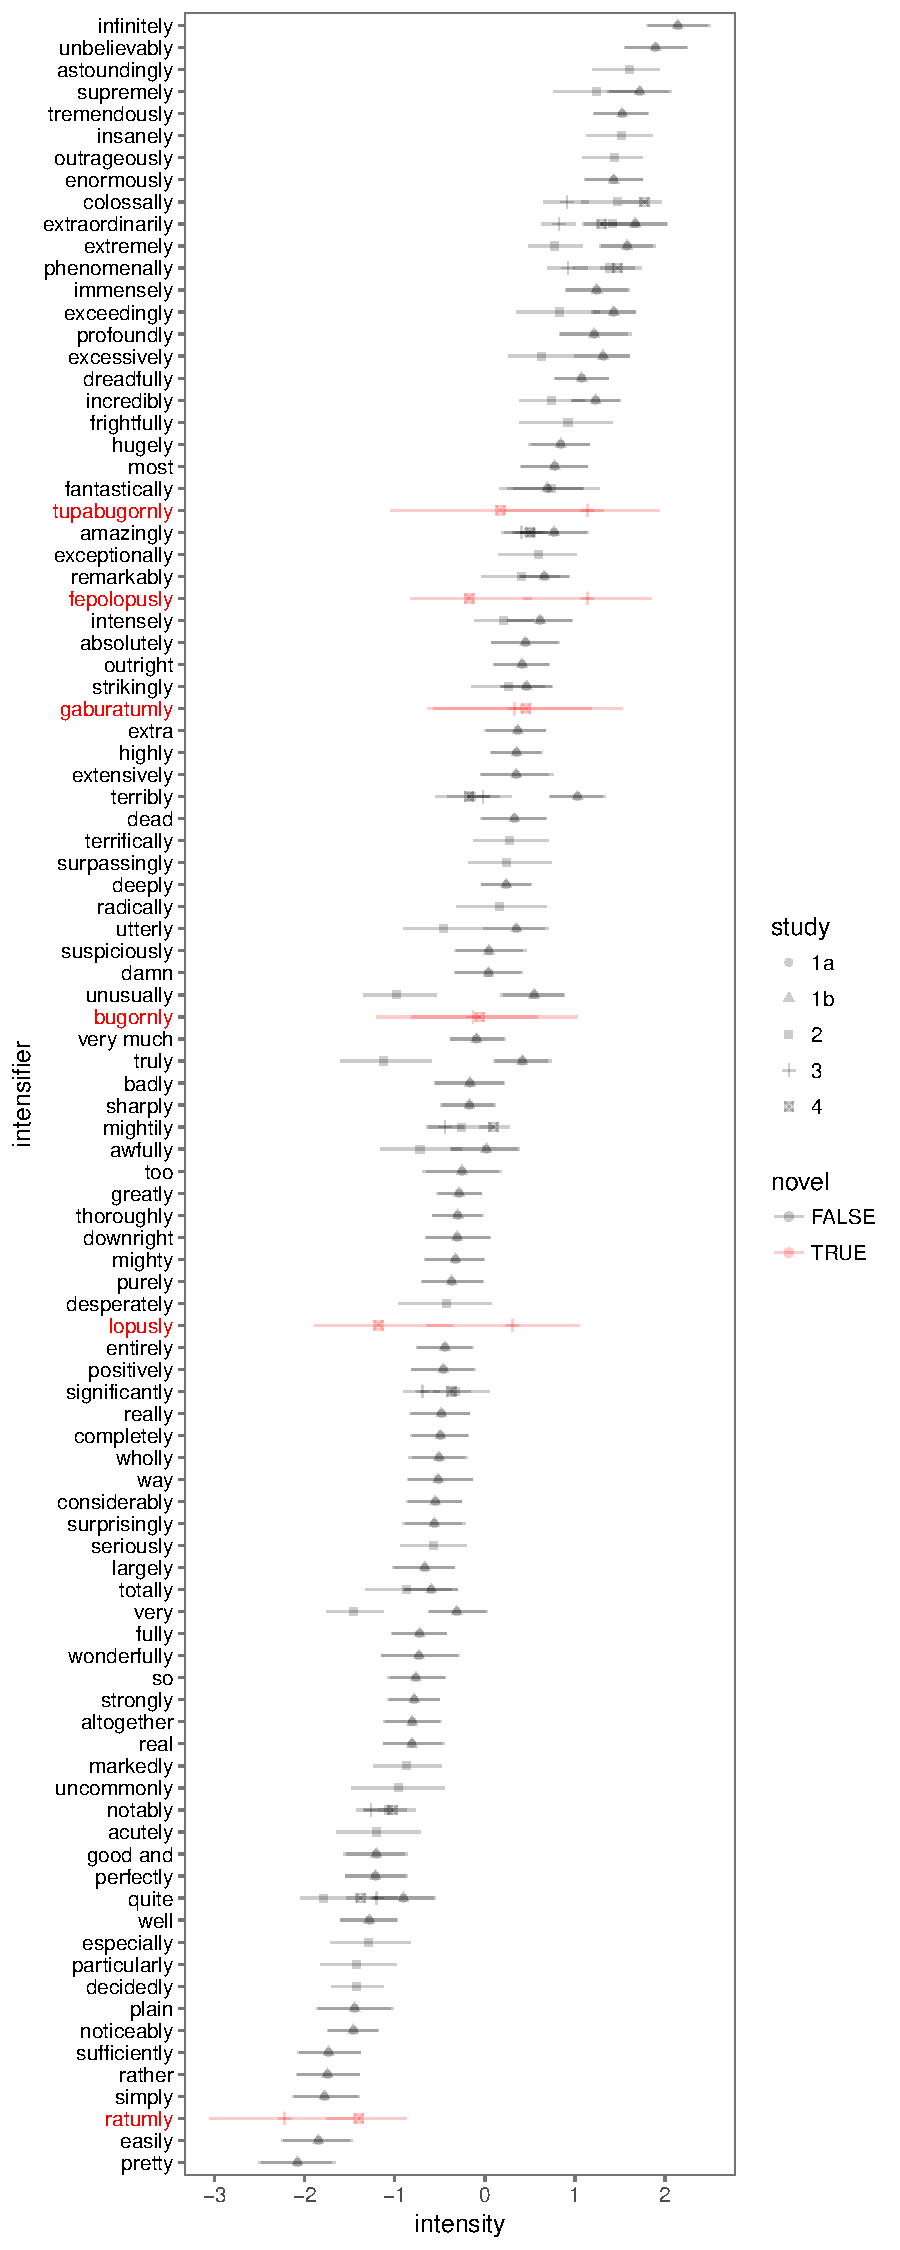
\includegraphics[width=0.5\textwidth]{images/intensities.pdf}
\end{center}
\caption{Intensities (each dependent measure, z-scored) of all intensifiers across all 5 studies. Novel intensifiers are shown in red, standard English intensifiers in black.}
\label{fig:intensities}
\end{figure}

\end{appendices}
